\documentclass[12pt]{article}
\usepackage{graphicx}
\usepackage{lipsum}
\usepackage[showframe=false]{geometry}
\geometry{verbose,tmargin=70 pt,bmargin=70 pt,lmargin=90 pt,
rmargin=90 pt}
\begin{document}
\begin{titlepage}
\begin{center}
\line(1,0){300}\\
[0.25 in]
\huge{\bfseries EFFICIENT PARALLELIZATION OF CYK PARSING ALGORITHM}\\
[0.1 cm]
\line(1,0){200}\\
[0.5 cm]
\textsc{\large Department of Computer Science Engineering}\\
\textsc{\large University of Central Florida}\\
\end{center}
\vspace{8 cm}
\begin{flushright}
\textsc{ \large Manasa Kashyap Harinath\\
         Muhammad Irtaza Safi\\
         Sravanthi Avasarala\\}
\end{flushright}
\end{titlepage}
\begin{abstract}

\large CYK algorithm is a Natural Language parsing algorithm which is named after its inventors Cocke–Younger–Kasami algorithm (also called as CYK algorithm) is used to parse Context free grammars. CYK algorithm requires the grammar to be in the Chomsky Normal Form. It is one of the most efficient parsing algorithms we have. The sequential CYK algorithm records a complexity of O(n3)during a worst case scenario, where ‘n’ is the length of the string to be parsed by CFG. In this paper we try to implement the CYK algorithm on multiple processors and compare the performance against its sequential counterpart.
\end{abstract}

\vspace{50 cm}
\section{Introduction}
Natural Language Processing is the field of Artificial Intelligence and Machine Learning which is concerned with the automated interaction between Human language (Natural) and computers. The objective is to make computers understand and process the natural or human language.There are various algorithms designed to achieve this objective.
However, Natural Language Processing(NLP) algorithms are among the most computationally-challenging and time-consuming algorithms in computer science. In order to handle natural languages, large statistical grammar models and lexicons have to be built and consulted throughout NLP algorithms. The quality of NLP algorithms is directly proportional to the sizes of these statistical models, where large ones can consist of billions of words and grammar rules. Therefore, it is inevitable but to compromise on the time complexity to obtain good results.
In our paper, we consider one of the most popular Natural Language processing algorithms, Cocke-Kasami-Younger (CYK). It is a bottom up parsing algorithm which expects the grammar to be in CNF, Chomsky Normal form. Parsing a CYK algorithm is time consuming as the Natural language grammars are very large. Since performance is the major concern, this gives us opportunity to exploit the concepts of multi thread programming . In order to take advantage of such hardware, however, algorithms must be redesigned to divide work into largely independent parts. Thus, we intend to demonstrate another implementation of CYK algorithm using parallel processing.
\section{Related Works}
In order to improve the effectiveness of the algorithm, several attempts to their parallelization have been proceeded. A sequential CYK algorithm executes with $O(n3)$ complexity. S.Kosoraju and J Chang proposed a parallel algorithm of a two dimensional array of $n^2$ finite state machines which yields a O(n) complexity\cite{a}\cite{b}. However, they assumed that the number of processors is proportional to the length of the input string ‘w’.

\vspace{2 mm}


A.Niholt \cite{c} proposed a parallel version of Tabular CYK in which each processor is responsible for computing the values of each cell. In his proposal, it was assumed that the processing units of one level depend on the results of the processing units which are lower than them. However, this model proposed by A.Niholt was considered as a theoretical contribution. Our approach is similar to the one that A. Niholt had proposed.

\vspace{2 mm}
 
Thompson (1994) pointed out that the close relationship between CYK parsing and matrix multiplication can be exploited for parsing in parallel.


\vspace{2 mm}
O. Ibara \cite{d}proposed an algorithm which is very similar to that of A. Niholt’s. In this approach, the of processors are lesser than the number of tasks. This approach has a processor mapped to a column in the chart instead of a single cell. This decreases the cost of communication between the processors.



\section{Background}
A formal language is a set of strings of symbols that are restricted by the rules which are specific to it. An alphabet of a formal language is the set of symbols or letters from which the strings of the language are formed. A formal language L is a possibly infinite set of strings over a finite alphabet $\Sigma$. The strings from these alphabets are called words and the words of the formal language are called well-formed language.\cite{e}The field of formal language theory studies mainly about syntactical aspects and regularities of natural languages.  The term syntax is used to refer the study principles, rules and processes that govern the structure of sentences. 
\subsection{Grammar}
Grammar is a set of formal statements which is used to prove that a string ``a" satisfies certain  assumption. It can also be described as set of rules for putting strings together which further corresponds to a language. For example, if we can prove a string ``a" with respect to the language L, then we would conclude that ``a" is in L, i.e. a $\varepsilon$ L. Grammars indicates how to transform a start symbol S, into a string of symbols. Grammars are of different types such as, right-linear or Type 3, context-sensitive grammar, etc. In our paper we consider context-free grammar or Type 2 grammar. In CFG, the rules are of the form A $\rightarrow$ $\psi$, where A is a single non-terminal element and $\psi$  is a string of terminals or non-terminals.
\subsection{Parsing}
Parsing or syntactic analysis is the process of analysing the string of symbols of any language, conforming to the rules of a formal grammar,L(G).  It is often performed as a method of understanding the exact meaning of a sentence or a word. In another words, it is a process of breaking down an entity into meaningful parts using a definable common sets called  ``definitions". The task of the parser is mainly to figure out how to derive the input from the start symbol of the grammar. Essentially, this can be done two ways:\\
1){\bf Top down approach}: This parsing starts from the root of the parse tree and grow down towards  the leaves.\\
2) {\bf Bottom up approach}: This parsing starts from the leaves and grow towards root.\\
A context-free grammar (CFG) is a set of productions used to generate pattern of strings. The components of CFG are variables, terminals,productions. A non-terminal symbol is any symbol we use in the grammar that cannot be a final string. In the grammar below, ``S" and ``A" are non-terminal symbols, and ``0" and ``1" are ``terminal" symbols.\\

\vspace{20 mm}
\begin{center}
S$\rightarrow$AA\\
A$\rightarrow$0\\
A$\rightarrow$1\\
\end{center}
\vspace{10 mm}
We can provide a formal definition of a context free grammar. It is a 4-tupple (V,$\Sigma$, S, P) where:\\
1) V is a finite set of variables \\
2) $\Sigma$ is a finite alphabet of terminals\\
3) S is the start variable and\\
4) P is the finite set of productions.\\ Each production has the form V $\rightarrow$ (V $\bigcup$ $\Sigma$)$\ast$.
\subsection{Chomsky Normal Form}
Chomsky Normal Form is used to answer questions about  the context-free languages. A grammar where every production is either in the form A $\rightarrow$ BC or A $\rightarrow$d (where A, B, C are arbitrary variables and d an arbitrary symbol) is said to be in CNF. If language contains $\epsilon$ , then we produce S $\rightarrow$ $\epsilon$ where S is start symbol. The main purpose of using CNF is that, for every derivation of string of n letters, it produces exactly $2n-1$ steps. One can convert any grammar into CNF in four steps:\\
1)Get rid of all ε productions.\\
2) Eliminate variable unit productions.\\
3) Replace every production that are too long by shorter productions.\\
4) Move all terminals to unit productions.\\
\section{CYK Algorithm}
CYK (Cocke–Younger–Kasami ) algorithm is mainly used to parse the grammar which is in Chomsky normal form(CNF). It uses ``dynamic programming” or ``table-filling" algorithm which usually follows bottom up approach. The term dynamic programming usually describes the process of saving partial solutions inside the cell table. It is one of the earliest recognitions and parsing algorithm which mostly recognizes the languages that are defined by context-free grammar.
This algorithm considers every possible consecutive subsequence of letters and sets K $\varepsilon $ T[i,j] if ,the sequence of letters starting from i to j is generated from the non-terminal K.  Once it has considered sequences of length 1, it increments to sequences of length 2 and so on.  For subsequence of length 2 and greater, it considers each and every possible partition of the subsequence into two halves, and checks if there is a production A$\rightarrow$BC, such that B matches the first half and C matches the second half. In a simpler way ,the solution to the problem A[i,j] can be split into A[i,k] and A[k,j].This algorithm solves the problems using a table data-structure called the chart.

\vspace{30 mm}
\subsection{Construction of a Triangular table:}
1)	$X_i$,is the set of variables A such that A$\rightarrow$wi is a production of G.\\
2)	Compare at most n pairs of previously computed sets:
$(X_{i,i}, X_{i+1},_ j )$, $(X_i,_ {i+1} , X_{i+2},_ j )$ $\cdots$ $(X_i,_ {j-1} , X_j,_ j )$

\vspace{10 mm}

\includegraphics{capture.png}\\
\subsubsection{Example}
Consider the following string w=‘baaba’. Let us check if the string ‘w’ satisfies the grammar L(G) below:\\
1)	S $\rightarrow$ AB $\mid$ BC\\
2)	A $\rightarrow$ BA $\mid$ a\\
3)	B $\rightarrow$ CC $\mid$ b\\
4)	C $\rightarrow$ AB $\mid$ a\\
Now, we start the processing from the bottom row of the table. For each character in the string, corresponding rules are checked and is written in the chart as shown below:

\vspace{10 mm}

\includegraphics{capture1.png}\\
$X_1,_2$ = $(X_i ,_i,X_{i+1} ,_ j)$ = $(X_1 ,_ 1   , X_2 ,_ 2)$\\
  =\{B\} \{A,C\}\\
  = \{BA, BC\}\\
  
  \vspace{1 mm}
Look for production rules to generate BA or BC in L(G):\\
Hence, $X_1,_2$=\{S,A\}\\
Similarly, we compute $X_2,_3$, $X_3,_4$,$ X_4,_5$

\vspace{10 mm}

\includegraphics{capture2.png}\\

To process the combinations for the next level, we compute the following:\\
$X_1 , _3 $	= $(X_i ,_i ,X_{i+1} , _j)$ $(X_i , _{i+1} ,X_{i+2} , _j$)\\  
	        = $(X_1, _1, X_{2,3})$ , $(X_1,_ 2,X_3,_ 3)$\\
\{B\}\{B\} $\bigcup$ \{S, A\}\{A, C\}= \{BB, SA, SC, AA, AC\}\\
Since none of the combinations matches the ones in the L(G), $X_1,_3$= $\phi$.\\
Similarly, we compute the rest of the cells by using the values in cells which are one step lower than the current cell.\\

  
After computing values of all the cells using the steps specified above, we get:


\includegraphics{capture5.png}\\

Since$ X_1,_5$ =\{S,A,C\} is present in the grammar L(G), we say that the string ``baaba" is present in the grammar L(G).

\section{Our Approach and Implementation}
 By the time of our midterm submission we had implemented one parallel approach to the CYK parsing algorithm. We stated then that we would experiment with a few other approaches and that we would try to speed up grammar rule parsing by implementing a concurrent MultiMap data structure. \\
 
 
 The following is an excerpt from our midterm report: \\	
 
 \vspace{2 mm}
\textit{
\footnotesize{	
\textbf{\textit{``We have implemented a sequential as well as one version of a parallel program for the CYK algorithm }}and are exploring various approaches to parallelize the algorithm. Below, we discuss various ideas for parallelizing our sequential program and then explain one of the approaches that we\textsc{\char13}ve taken. Our sequential program can be thought of as operating in a two-step process: \\
1)	Parsing the grammar.txt file and loading it into memory.\\
2)	Running the algorithm. \\
Step 1 can obviously be parallelized but it\textsc{\char13}s complexity depends on the data-structures being used to store the grammar. We are currently using a variant of a Hash Map called MultiMap (Provided in Google\textsc{\char13}s Guava Library) which allows for one to many mapping (very useful for storing grammar rules). The hash-map is needed because it provides O (1) access during the evaluation of the algorithm so we cannot replace it with a concurrent list or array which will cause a slow down when the size of the grammar is huge. However, when parsing huge grammars, we would like multiple threads to take on the workload while remaining efficient.\textbf{\textit{ Therefore, we propose a concurrent implementation of a MultiMap which introduces a significant level of parallelism by only serializing writes to the same key rather than locking down the whole structure.}}This can be achieved by having a list of locks and requiring any write to first acquire a random lock from that list or keep traversing the list until a lock becomes available....."
}
}

	\vspace{2 mm}
After further exploration, we found that building a concurrent MultiMap data-structure would be an infeasible and unpractical exercise for two reasons: \\
1)	Parsing is a one-time process and not a part of the dynamic programming CYK algorithm.\\
2)	To synchronize writes to the same key, we would have to introduce additional processing which will end up delaying the whole process. 

\vspace{5 mm}
{\bf Therefore, we choose to ignore the parsing step and choose instead to focus on parallelizing the core algorithm.}  \\
In the following sections, we list our approaches as well as their evaluations on input strings of different sizes. \\
\subsection{Serial (Single Threaded) CYK algorithm}
This is the generic single threaded CYK algorithm implemented in the file CYK.java. The triangleTable class is the two-dimensional table that is iteratively built up by the algorithm. Each table index (i,j) is a tableItem object which stores the computation results for the index (i,j). Please refer to the CYK description in the previous sections for more detail. The CYK algorithm being dynamic programming, is inherently not a parallel algorithm as each step is dependent on the result of some previous step. The serial implementation evaluates the table one row at a time (left to right), this means that all dependencies for an index are already resolved before the index itself is attempted. \\
Two kinds of parallelism can be exploited to enhance the CYK algorithm.\\
1)	Inter-cell parallelism\\
2)	Intra-cell parallelism\\
Intra-cell computations are small but numerous therefore there is a danger of offsetting any benefits of parallelization by the amount of time spent managing/allocating thread resources and context switching. Therefore, our first approach was to try and attempt inter-cell parallelism. 
\subsection{Parallel ‘Ladder Climbing’ CYK algorithm}
We have implemented a Lock-Free ``ladder climbing" algorithm given in \\
{\bf CYK{\_}PARALLEL.java} similar to [5]. For this approach, we only exploit inter cell parallelism. Given the string given above in the example (``baaba"), we allocate the responsibility of filling the specific character\textsc{\char13}s column to a thread. Therefore, we have L number of threads for any arbitrary string of length L. Instead of going for locks we choose to use atomic operations. As seen in the example of CYK given above, to evaluate a block one must first evaluate all its dependencies i.e.  one must know all the blocks directly below it and all the blocks diagonal (bottom-right) to it. In a serial algorithm, the dependencies are already evaluated since the algorithm proceeds row wise one block at a time. However, in the multi threaded version we can only guarantee the availability of the vertically below dependency since we know the thread evaluating a block has already evaluated all its vertical dependencies. The diagonal dependencies have to be evaluated by other threads and therefore a thread waits using a compareAndSet loop on a ``resolved" Atomic Boolean value in the tableItem class. Once a table item has been computed, the computing thread uses an atomic compareAndSet to set resolved to ``true" hence making it accessible to the waiting threads.\\
\subsection{Parallel Ordered Jobs CYK algorithm \\ (CYK{\_}PARALLEL{\_}TWO.java)}
As we show later in our evaluation section, the first approach is not optimal because of two reasons:

\vspace{5 mm}
1)Creating a thread for every column creates a massive overhead. \\

2)A lot of time is spent waiting on dependencies being evaluated by other threads. \\

\vspace{5 mm}
In our midterm report, we stated that we would implement a global job scheduler that would ask waiting threads to help in computing their dependencies. We think this approach would not be much better than approach one because it would still have the same number of threads plus the added complexity of synchronizing the data structure containing the jobs.
Instead we implemented a much simpler approach as we made a \textit{lucky insight} when inspecting the table. From the table, we can note that all the indexes in the same row DO NOT depend on each other. This gives us the perfect opportunity to parallelize by having threads first solve all items in the same row. We do this by giving an increasing job priority to each index while traversing the table row-wise (left to right) and then sorting the jobs by the job priority. Since each row such as [A, B, C, D, E] will have priority [x, x+1, x+2, x+3, x+4, x+5] (each element represents the individual priority of the item) and a priority of zero is the maximum possible, our threads will now solve jobs in a manner which causes minimal waiting. Furthermore, we now have the benefit of not having to create a thread for every character in the input string. \\

\vspace{70 mm}
\subsubsection{Example}
Suppose the first two (bottom) rows of a triangle table as follows:
\textit{The alphabets are just labels for jobs to be done.}\\

[W, X, Y, Z] \\

[A, B, C, D, E] \\

Jobs A, B, C, D, E are not dependent on each other but W, X, Y, Z are dependent on the results of A, B, C, D and E. Therefore, we can parallelize A, B, C, D and E and then W, X, Y, Z without any need for complex synchronization. If a thread reaches W while E is still being evaluated, then it can still wait on the evaluated atomic Boolean. The likelihood of waiting however is significantly reduced and the situation where 1 thread is waiting for the next, which is in turn waiting for the next and so on (very likely in algorithm 1) will rarely occur.
\subsection{Parallel ``Ordered Jobs" with Intra cell parallelism\\(CYK{\_}PARALLEL{\_}THREE.java)}
As we stated in our midterm report, there are several unrelated computations that happen when computing a single table index which can be parallelized. \\


The following is an excerpt from our midterm report: \\

\textit{
\footnotesize	{
``This requires the computation of the cell to be split into discrete segments which can later be combined into a single operation. Fortunately, the computations required for this algorithm present a clear opportunity for that!\\ The following steps must be carried out when evaluating a block: \\
1)List all the vertical dependencies (all the blocks below it)\\
2)List all the diagonal dependencies (all the blocks in the diagonal leading down and right from a block). Refer to the example above for more clarity.\\
3)Multiply the corresponding entries in the vertical and diagonal dependencies.\\
4)Perform a union of the multiplication results from 3.\\
5)Reduce the final result by applying grammar rules.\\
Task 3 is the most computationally intensive, especially for huge grammars. Fortunately, each individual multiplication is self-contained and can therefore be delegated to other threads....."}}

\vspace{5 mm}
In this version, we modify the ``Ordered Jobs" algorithm to include intra-cell parallelism. We avoid spawning new threads for every block by making use of Java\textsc{\char13}s Executor Service as well the excellent JAVA 8 Callable$<$ T $>$ and Future $<$T$>$ API. We separate the multiplication jobs by immediately assigning it to an executor thread as soon as it is finalized. We then wait for our ``Future" tasks to return before proceeding with the Union operation. The union operation operates over multiple sets and as such there isn\textsc{\char13}t any need to parallelize it. Unfortunately, at least on our test bed of a dual core (Core i5) MacBook Pro, this algorithm does not yield significant advantages over the second one and is many cases worse as we increase the number of threads available to help in intra-cell computations.


\vspace{5 mm}
\section{Evaluation}
\subsection{Platform: Dual Core (Core i5) MacBook Pro 13}
Since this is a dual core machine, we expect optimal performance with two threads. 
We perform tests by varying the length of the string to be identified as part of the grammar or not. Increasing the string length drastically increases the number of jobs and hence the size of the table. Our evaluation starts with comparing our best performing algorithm (CYK Ordered Jobs) and then goes to the worst performing (Ladder climbing) algorithm.\\


Note: We decided to implement and compare our own versions to promote learning and understanding of the problem rather than wholesale copying a research paper. We felt that in the timespan of a semester, figuring out implementations ourselves would be much more effective in helping us learn. The most efficient algorithms for CYK are on CUDA and therefore we were not able to compare our implementations with others out there.
\subsubsection{CYK Serial compared with CYK Ordered Job (2 threads)}

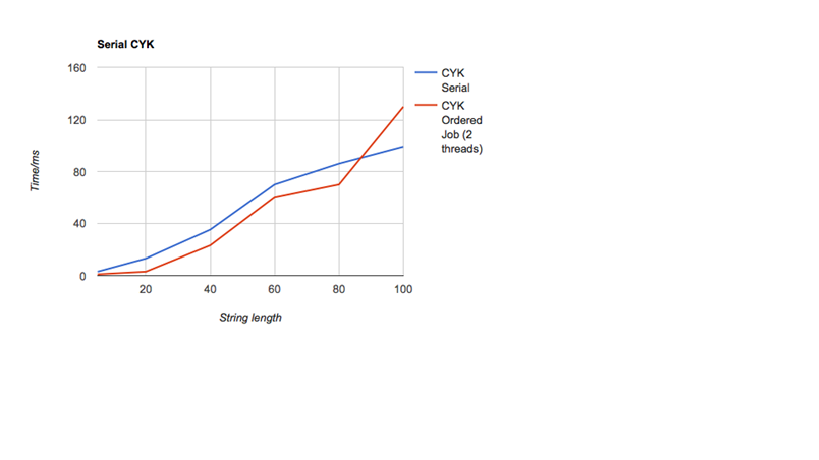
\includegraphics{file1.png}

\vspace{30 mm}
As seen in the graph, the parallel ordered job version outperforms the serial algorithm for strings up to length 80. We aren\textsc{\char13}t completely sure why the performance suddenly falls after length 80 , however we suspect that the ``getQueuedJob()" method might be taking too long to return since the number of jobs increase substantially with a single increment in string length. \\
\subsubsection{CYK Serial, CYK Ordered Job (2 and 4) threads}

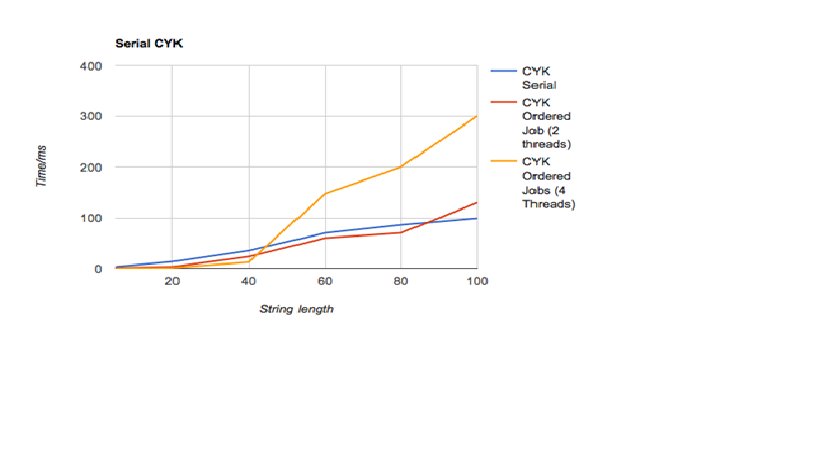
\includegraphics{file2.png}\\

As stated above, increasing the number of threads creates a big overhead and performance deteriorates. This is not expected to be the case on processors which can have more CPUs and can thus handle a larger number of concurrent threads without switching between them.
                             
\subsubsection{CYK Serial and Ordered Job compared with CYK Intra cell}

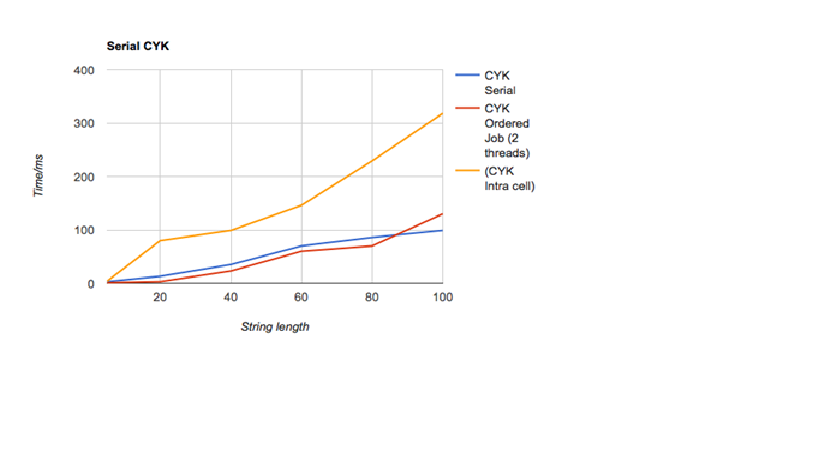
\includegraphics{file3.png}\\
Here, we see that the intra cell parallelism creates overhead which is not worth it. Performance is much worse from the get go. We tried various combinations of number of threads and the graph obtained above is the best performance we could get on our test machine. Since we used Java\textsc{\char13}s executor service and Future API, it is possible that a large overhead is being introduced because of their inner workings. However, if we had used the default threads and assigned them jobs at each index that would have created even more overhead. \\
Finally, we compare our first parallel algorithm (Ladder Climbing) with the rest. We see that this is an exceptionally bad parallel implementation.\\

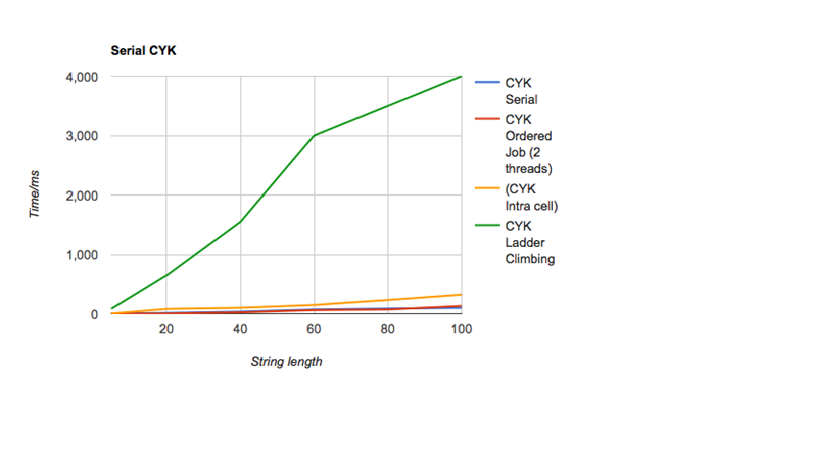
\includegraphics{file4.png}\\

\section{CONCLUSION}
The best performing algorithm for us is the CYK Ordered Job algorithm (2 threads). We believe the CYK algorithm cannot be trivially parallelized since it’s structure is inherently serial. Architectures which can handle a huge number of threads i.e CUDA are better suited for parallel CYK implementations. 


\vspace{70 mm}

\begin{thebibliography}{1}
\bibitem{a} Kosoraju, S. (1975). Speed of recognition of context-free languages by array automata. SIAM Journal on Computing, 331-340.
\bibitem{b} J. H. Chang, O. H. (1987). Parallel Parsing on a One-Way Array of Finite-State Machines. IEEE Transactions on Computers, 64-75.
\bibitem{c} Nijholt, A. (1990). The CYK-approach to serial and parallel parsing. Language research, 229-254.
\bibitem{d} O.H. Ibarra, T. P. (1991). Parallel recognition and parsing on the hypercube. Computers, IEEE Transactions on,, 64–770.
\bibitem{e} J. E. Hopcroft, R. M. (2001). Introduction to Automata Theory, Languages and Computation, second Edition, Addition Wesley.
\end{thebibliography}


\end{document}
